\documentclass[12pt]{article}

\usepackage[affil-it]{authblk}
\usepackage{hyperref}
\usepackage{braket}

\usepackage{amsmath,amssymb,amsthm}
\usepackage{esint}
\usepackage{bm}
\usepackage{graphicx}
\usepackage{caption}
\usepackage{subcaption}
\usepackage[margin=0.9in]{geometry}
\usepackage[all]{xy}
\usepackage{algorithm}
\usepackage{amsthm}
%\usepackage{cite}
\usepackage{titlesec}
\usepackage{hyperref}

\usepackage{algorithm,algpseudocode,float}
\usepackage{color}
\usepackage{tikz}
\usetikzlibrary{shapes.misc,shadows, arrows, shapes, intersections}

\usepackage[sort&compress,square,comma,authoryear]{natbib}

\setcounter{secnumdepth}{4}

\titleformat{\paragraph}
{\normalfont\normalsize\bfseries}{\theparagraph}{1em}{}
\titlespacing*{\paragraph}
{0pt}{3.25ex plus 1ex minus .2ex}{1.5ex plus .2ex}


\newcommand{\doi}[1]{\href{http://dx.doi.org/#1}{doi:\texttt{#1}}}
\newcommand{\arxiv}[1]{\href{http://arxiv.org/abs/#1}{\texttt{arXiv:#1}}}
\newcommand{\urlprefix}{}

\theoremstyle{plain}
\newtheorem{theorem}{Theorem}[section] % reset theorem numbering for each section

\theoremstyle{definition}
\newtheorem{definition}{Definition}[section]
\newtheorem{exmp}{Example}

\newcommand{\floor}[1]{\lfloor #1 \rfloor}
\newcommand{\ceil}[1]{\lceil #1 \rceil}

% \usepackage{mathtools} 
% \DeclarePairedDelimiter\ceil{\lceil}{\rceil}
% \DeclarePairedDelimiter\floor{\lfloor}{\rfloor}

% thanks to https://tex.stackexchange.com/users/5764/werner for breakable algorithm
% https://tex.stackexchange.com/questions/33866/algorithm-tag-and-page-break

\makeatletter
\newenvironment{breakablealgorithm}
{% \begin{breakablealgorithm}
	\begin{center}
		\refstepcounter{algorithm}% New algorithm
		\hrule height.8pt depth0pt \kern2pt% \@fs@pre for \@fs@ruled
		\renewcommand{\caption}[2][\relax]{% Make a new \caption
			{\raggedright\textbf{\ALG@name~\thealgorithm} ##2\par}%
			\ifx\relax##1\relax % #1 is \relax
			\addcontentsline{loa}{algorithm}{\protect\numberline{\thealgorithm}##2}%
			\else % #1 is not \relax
			\addcontentsline{loa}{algorithm}{\protect\numberline{\thealgorithm}##1}%
			\fi
			\kern2pt\hrule\kern2pt
		}
	}{% \end{breakablealgorithm}
		\kern2pt\hrule\relax% \@fs@post for \@fs@ruled
	\end{center}
}
\makeatother

\algnewcommand\algorithmicforeach{\textbf{for each}}
\algdef{S}[FOR]{ForEach}[1]{\algorithmicforeach\ #1\ \algorithmicdo}

\titleclass{\subsubsubsection}{straight}[\subsection]

\newcounter{subsubsubsection}[subsubsection]
\renewcommand\thesubsubsubsection{\thesubsubsection.\arabic{subsubsubsection}}
\renewcommand\theparagraph{\thesubsubsubsection.\arabic{paragraph}} % optional; useful if paragraphs are to be numbered

\titleformat{\subsubsubsection}
{\normalfont\normalsize\bfseries}{\thesubsubsubsection}{1em}{}
\titlespacing*{\subsubsubsection}
{0pt}{3.25ex plus 1ex minus .2ex}{1.5ex plus .2ex}

\makeatletter
\renewcommand\paragraph{\@startsection{paragraph}{5}{\z@}%
	{3.25ex \@plus1ex \@minus.2ex}%
	{-1em}%
	{\normalfont\normalsize\bfseries}}
\renewcommand\subparagraph{\@startsection{subparagraph}{6}{\parindent}%
	{3.25ex \@plus1ex \@minus .2ex}%
	{-1em}%
	{\normalfont\normalsize\bfseries}}
\def\toclevel@subsubsubsection{4}
\def\toclevel@paragraph{5}
\def\toclevel@paragraph{6}
\def\l@subsubsubsection{\@dottedtocline{4}{7em}{4em}}
\def\l@paragraph{\@dottedtocline{5}{10em}{5em}}
\def\l@subparagraph{\@dottedtocline{6}{14em}{6em}}
\makeatother

\setcounter{secnumdepth}{4}
\setcounter{tocdepth}{4}


\begin{document}
	\title{Algorithm to find Maximum Clique}
	\author[1]{Subramaniyan Neelagandan\footnote{Email: subramaniyan.neelagandan@outlook.com; web: https://github.com/SubbuN/Clique}}
	
	\date{}
	\maketitle

\begin{abstract}
	A new constructive, practical algorithm is presented here to find whether a given graph $G(V,E)$ has clique of size $k$, maximum clique size, counting number of maximum cliques, and enumerating all maximum cliques. Algorithm returns a certificate containing maximum clique size $\omega(G)$ and an instance of clique of size $\omega(G)$.
	
	We present how the number of maximum cliques can be counted efficiently without doing one by one. Also presented here is how we can enumerate all maximum cliques efficiently rather than doing individually.
\end{abstract}

%\tableofcontents

\section{Introduction}
Finding maximum clique size for a given graph $G(V,E)$ is so far hard. This prevented us from moving forward and gain any knowledge about this problem and related problems. The presented algorithm breaks through this hardness and helps us move forward.

Provided algorithm solves 
\begin{itemize}
	\setlength{\itemsep}{0pt}
	\setlength{\parskip}{0pt}
	\setlength{\parsep}{0pt}
	\item any complete multipartite graph instances under $O(n^3)$.
	\item in polynomial time when input graph has clique of size $k$ with $N$ vertices where $N < 2k$ and input graph has no vertices that is connected to all vertices in the graph.
	\item rest of graphs are solved with quasi polynomial time for up to 1000+ vertex graph into sub-exponential for large graphs.
	\item The best case complexity is $O(n^2)$.
\end{itemize}


\section{Terminology}
Following building blocks are used throughout this paper.

\subsection{Neighbourhood graph N(v)}
\begin{definition} \label{NeighbourhoodGraph}
	Let G(V,E) be a undirected graph. Neighbourhood graph N(v) of vertex v in G is the induced subgraph of G consisting of all vertices adjacent to v.
\end{definition}

\fbox{\parbox{\dimexpr\linewidth-2\fboxsep-2\fboxrule\relax}{
		Maximum clique size consisting vertex v in graph G is 1 plus maximum clique size of \\
	neighbourhood graph N(v).
}}


\subsection{Partition}
\begin{definition} \label{Partition}
	Let G(V,E) be an undirected graph. Partition P is an independent set S such that $\exists v \in S$
	 whose  $N(v) \equiv V - S$
\end{definition}

\fbox{\parbox{\dimexpr\linewidth-2\fboxsep-2\fboxrule\relax}{
	Maximum clique size of graph G when a partition could be extracted is 1 for partition P plus maximum clique size of G(V - S, E).
}}

\subsection{Clique}
\begin{definition}
Clique is an undirected graph G(V,E) where each vertex has an edge connected to every other vertex in the graph.
\end{definition}

\fbox{Clique is a trivial complete multipartite graph.} \ref{Clique}

\subsection{Maximum Clique}
\begin{definition}
A maximum clique of an undirected graph G(V,E) is a clique of maximum possible size for G(V,E).
\end{definition}

\subsection{Active Graph $G_a$}
\begin{definition}
	Let G(V,E) be an undirected graph. Let T be set of vertices that are already explored. Active graph is defined as $G_a(V-T,E)$.
\end{definition}

\subsection{Proper Complete Multipartite Graph} \label{ProperCompleteMultipartiteGraph}
\begin{definition}
	A proper complete multipartite graph is a complete multipartite graph in a set of complete multipartite graphs that can not be combined with another complete multipartite graph in the set to form a new complete multipartite graph.
\end{definition}

Let set of elements S be \{1, 2, 3, 4, 5\}. \\
Let set of complete multipartite graphs $S_c$ be $\{\{\{1\},\{2\},\{3\}\}, \{\{1\},\{2\},\{4\}\}, \{\{2\},\{3\},\{5\}\}\}$. In set $S_c$, none of the complete multipartite graphs are proper. Set \{\{1\},\{2\},\{3\}\} can be combined with \{\{1\},\{2\},\{4\}\} to form \{\{1\},\{2\},\{3, 4\}\}. Similarly, set \{\{1\},\{2\},\{3\}\} can be combined with \{\{2\},\{3\},\{5\}\} to form \{\{1,5\},\{2\},\{3\}\}. Therefore $S_c$ can be rewritten either as $\{\{\{1\},\{2\},\{3, 4\}\}, \{\{2\},\{3\},\{5\}\}\}$ or $\{\{\{1,5\},\{2\},\{3\}\}, \{\{1\},\{2\},\{4\}\}\}$. Both forms of rewritten sets are proper complete multipartite graphs since none of set members can be combined with another one in that set.

\subsection{Fence Graph} \label{FenceGraph}
Fence graph is a graph that looks like a fence when drawn on 2-dimensional geometry.

How to construct a fence graph?

Let $N$ be the number of vertices. Chose a height $h$ of the fence such that $(2 \times h) < N$. Now place all vertices on a circle in unit distance apart. For each vertex, create edges to connect $h$ vertices on its right and $h$ vertices on its left. 

How to draw this graph in a 2-dimensional geometry?

For each vertex, draw one line on its right from (0,v) to (h, v+h)  and one line on its left from (0,v) to (h, v-h). When all the edges are drawn, it forms a cylindrical fence. Cut vertically at any one point. Now it forms a 2-dimensional fence having all vertices marked at the bottom.


\begin{center}
	{\large Fence graph }
	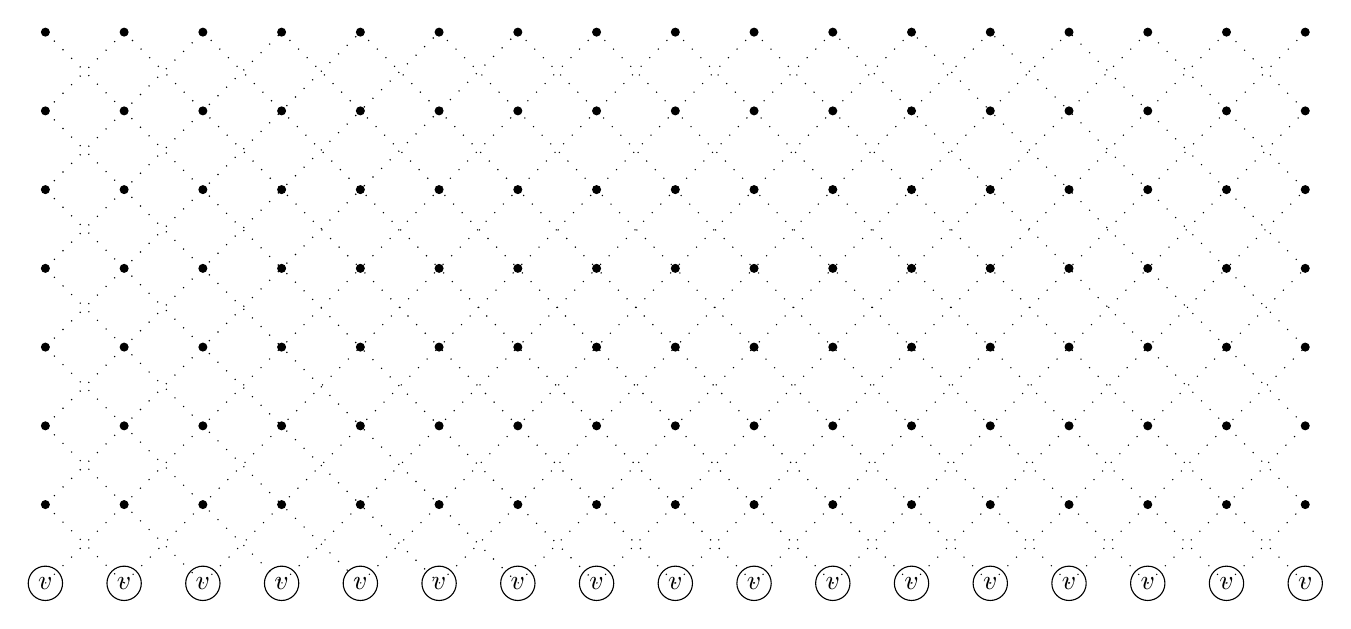
\begin{tikzpicture}
	\def\n{16}
	\def\k{7}
	\pgfmathparse{\n - \k - 1} \let \diff \pgfmathresult
	\foreach \x in {0,1,...,\n}{
		\node[draw,circle,inner sep=2pt] at (\x, 0) {$v$};
		\foreach \y in {1,2,...,\k}{
			\node[draw,circle,inner sep=1pt,fill] at (\x,\y) {};
		}
	}
	\foreach \x in {1,...,\k}{
		\draw[loosely dotted] (0, \k - \x) -- (\x,\k);
		\draw[loosely dotted] (\n - \x, 0) -- (\n, \x);
		
		\draw[loosely dotted] (0, \x) -- (\x,0);
		\draw[loosely dotted] (\n, \k - \x) -- (\n -\x, \k);
	}
	\foreach \x in {1,...,\diff}{
		\draw[loosely dotted] (\x, 0) -- (\x+\k,\k);
		\draw[loosely dotted] (\n - \x, 0) -- (\n-\x-\k,\k);
	}
	\end{tikzpicture}
\end{center}


Why it is important?

Maximum clique size of this fence graph is (h + 1). Every vertices forms multiple maximum cliques. This graph resists partition extraction when number of non adjacent vertices of each vertex is greater than 1. Once one of the vertex is searched, we can apply compatible neighbourhood graph(s) optimization \ref{NeighbourhoodGraphOptimization} to skip exploring all other vertices.

\subsubsection{$2 \times h + 1 = N$ or $2 \times h = N$}
When $2 \times h + 1 = N$ or $2 \times h = N$, it forms a complete (multipartite) graph of size $N$ with $\omega(G) = N$.

\subsubsection{$2 \times h + 1 = N - 1$}
When $2 \times h + 1 = N - 1$, it forms a complete multipartite graph having $\frac{N}{2}$ partitions and each partition having cardinality of 2.

\subsubsection{Partitioning Fence Graph} \label{FenceGraphPartition}
\begin{theorem}
	A fence graph G has $\ceil{\frac{N}{\floor{\frac{N}{h + 1}}}}$ partitions with partition size of $\floor{\frac{N}{h + 1}}$. The last partition may have fewer members when $N \not \equiv 0$ (mod (h + 1)).
\end{theorem}

\begin{proof}
	Each vertex $v$ in fence graph G is connected to $h$ vertices on its right and $h$ vertices on its left. All other vertices are non-neighbors for $v$. When a non-neighbor vertex $u$ is picked, it automatically eliminates its neighbors from being part of the partitions. The distance between vertex $v$ and the first non-neighbor vertex $u$ on either side is $h$. Since this is the case for every vertex $v$ in the fence graph $G$, group is formed with cardinality of $(h + 1)$. A partition can contain only one member from each group. Therefore the partitin size is $\floor{\frac{N}{h + 1}}$ ($\equiv \ceil{\frac{N}{2 \times h + 1}}$). This yields number of partitions as $\ceil{\frac{N}{\floor{\frac{N}{h + 1}}}}$.
\end{proof}

\subsection{Complement of k-Partite Graph (Clique Sets)} \label{CliqueSet}
The complement of complete multipartite graph is a collection of disconnected graphs each being their own maximum clique.

The complement of k-partite graph is a set of cliques connected to each other.

In both of the above cases, the partition becomes clique in the complement graph.

\section{Complete Multipartite Graph}

A complete multipartite graph is a graph that is complete $k$-partite graph for some $k$. A complete $k$-partite graph is a graph that has $k$ partitions and every vertex has an edge to every other vertices in the graph except vertices from its own partition.

\subsection{Vertex Grouping} \label{CMGVertexGroup}

\begin{equation}
v \in V, \forall u \in V
\left\{ 
\begin{array}{ll}
\mbox{part of independent set} & \mbox{if u $\&$ v are either same or not adjacent} \\
\mbox{part of neighbourhood graph} & \mbox{if u $\&$ v are adjacent} \\
\end{array} \right.
\end{equation}


\subsection{Partition}
Every partition in a complete multipartite graph satisfies definition \ref{Partition}.

\subsection{Independent Set (S)}
Every partition in a complete multipartite graph is an independent set.

\subsection{Trivial Independent Set}
Trivial independent set is a non empty partition that has exactly one vertex.

\subsection{Finding a Independent Set}
Using \ref{CMGVertexGroup}, finding an independent-set (S) is picking a vertex from the graph and then identifying all its partition members.

It is trivial to find partition members of vertex v. The partition members of vertex v are v plus all non adjacent vertices of it.

\subsection{Finding all Independent sets}
Identifying all partitions from a complete multipartite graph is also trivial. Pick a vertex v and extract its partition from graph. Repeat this process till the graph becomes empty. At this point, we have all partitions/independent-sets that are part of complete multipartite graph.

\begin{breakablealgorithm}
	\caption{Finding all Independent sets : O($n^2$)}
	\begin{algorithmic}[1]
		\Function{GetAllIndependentSets}{$G(V,E)$}
		\State $independentSets \gets \emptyset$
		\While {$(G \neq \emptyset)$}
			\State $v \in V$
			\State $nonAdjacentVertices \gets GetAllNonAdjacentVertices(G(V,E), v)$
			\State $independentSet \gets nonAdjacentVertices \cup v$
			\State $independentSets \gets independentSets \cup independentSet$
			\State $G \gets G \setminus independentSet$
		\EndWhile
		\State \textbf{return} $independentSets$
		\EndFunction
	\end{algorithmic}
\end{breakablealgorithm}

\subsection{Maximum Clique Size}
The maximum clique size of complete multipartite graph is number of partitions it contains.

\subsection{Total number of maximum cliques}
Total number of maximum cliques in a complete multipartite graph is product of each partition size.

\subsection{Storing in O(n) space}

A complete multipartite graph can be stored as an array where the array index being vertex identifier and its value is nothing but the partition identifier.

\subsection{Partition size to its member's edge count}

A vertex which is part of the smallest partition contains largest number of edges and a vertex that is part of largest partition contains smallest number of edges.


\subsection{Complete Multipartite Graph are Associative}
Let A, B \& C are partitions. The resultant complete multipartite graph out of A * (B * C) is same as (A * B) * C.

\subsection{Complete Multipartite Graph are Commutative}
Let A \& B are partitions. The resultant complete multipartite graph out of A * B is same as B * A.

\subsection{Vertex's neighbourhood graph N(v)}
Neighbourhood graph N(v) of a vertex is same as all other vertices in the same partition. That is all members of a partition shares same exact neighbourhood graph.

\subsection{Neighbourhood graph also a Complete Multipartite Graph}
Neighbourhood graph N(v) of a vertex is either $\emptyset$ when graph is singleton set or an another complete multipartite graph which contains all partitions minus the vertex's partition.

\subsection{Partition members are isomorphic to each other}
Since all vertices of a partition shares same neighbourhood graph, each member is isomorphic to one another.

\subsection{Trivial Complete Multipartite Graph (Clique)} \label{Clique}
A trivial complete multipartite graph is a graph whose partitions are all trivial as well.

The number of partitions in a trivial comple multipartite graph equals the number of vertices in the graph.

This is also known in general as Clique.

\subsection{The maximum number of cliques possible in a graph with $n$ nodes}
\citet{MM60} \citet{MoonMoser65} 

\begin{equation}
\mbox{If } n \geq 2, then f(n) =
\left\{ 
\begin{array}{ll}
3\textsuperscript{n/3} & \mbox{if $n \equiv 0$ (mod 3);} \\
4.3\textsuperscript{(n-4)/3} & \mbox{if $n \equiv 1$ (mod 3);} \\
2.3\textsuperscript{(n-2)/3} & \mbox{if $n \equiv 2$ (mod 3);} \\
\end{array} \right.
\end{equation}

The above question is stated differently as "What is the largest number which can be written as the product of positive integers that sum to n?" \citet{Vatter}

Here each number in the product represents size of a partition in a complete multipartite graph.

Below is an alternate simple proof.

\begin{proof}
	Identity value for multiplication function is 1. Multiplying 1 with as many 1's is still 1 even though the sum of these 1's could be up to $\infty$. Therefore we can't use 1 in product of positive integers. Both 2 \& 3 can not be split into parts without having 1 in them. Therefore 2 \& 3 becomes basic atomic numbers for this set. Any number higher than 3 can be broken in to parts without having 1 being one of them. If the broken parts are not 2 \& 3, then they can be broken further till they are represented exclusively using 2 and/or 3. Now when you take 6, this can be broken into two possible ways with either \{2,2,2\} or \{3,3\}. $2^3$ which is 8 that is less than $3^2$ being 9. Therefore, we can replace every three 2's in the set with two 3's. The final set may either have no 2 at all or single 2 or double 2's and rest being 3's if any. This final set is represented using the above equation.
	
	These numbers signify partition size (number of vertex) for graph. Identity value 1 signifies trivial partition with single vertex in it.
\end{proof}

\subsection{How to generate maximum number of Proper Complete k-partite Graphs in a graph with $n$ nodes and $\omega(G)$ = k?}

Split the n nodes into two groups. Take the first group of vertices and form as many proper complete k-partite graphs having non trivial partitions as possible. Now, for each vertices in the second group, create one trivial proper complete k-partite graph from each of the first group's proper complete k-partite graph.

Lets us say that first group formed P proper complete k-partite graph. Let us say that second group has N vertices. Therefore, the total number of proper complete k-partite graphs formed are $N \times P + P$.

Note: The second group could be empty. Then it just becomes P.

\textbf{Why this is important?}

\textbf{Because this sets the lower bound for finding maximum clique size in a graph.}

\section{Search optimization}
Set of optimizations that can be performed while searching for maximum clique is presented in this section. These optimizations reduce the search space exponentially.

\subsection{Partition Extraction}
In an arbitrary undirected graph G(V,E), if a partition can be extracted then we should extract it as it reduces the search graph into G(V-S,E).

\begin{theorem} \label{PartitionExtractionOptimizationTheorem}
	If a partition P can be extracted from an undirected graph G(V,E) then the partition must contain a vertex v with maximum degree.
\end{theorem}

\begin{proof}
	Let vertex v has maximum degree. If v forms independent set with its non adjacent vertices, then v is part of the partition and its adjacent vertices forms neighbourhood graph N(v) and it satisfies the definition of \ref{Partition}.
	
	Suppose vertex v does not have maximum degree. Then there exists $\Delta(G) - deg(v)$ edges that connects set of vertices that are not adjacent to vertex v. Therefore vertex v does not form independent set with its non adjacent vertices.
\end{proof}

If there are more than one vertex with maximum degree, then each vertex needs to be checked for whether it forms an independent set with its non adjacent vertices.

Note: Near perfect fence graphs have large number of vertices with maximum degree. Not all vertices may form partitions.

\begin{breakablealgorithm}
	\caption{Extract a partition if possible : O($n^3$)}
	\begin{algorithmic}[1]
		\Function{ExtractPartition}{$G(V,E)$}
		\State $maxDegreeVertices \gets GetAllVerticesWithMaximumDegree(G(V,E))$
		\ForEach{$v \in maxDegreeVertices$}
			\State $nonAdjacentVertices \gets GetAllNonAdjacentVertices(G(V,E), v)$
			\State $potentialPartition \gets nonAdjacentVertices \cup v$
			\If{(IsIndependentSet(potentialPartition))}
				\State \textbf{return} $potentialPartition$
			\EndIf
		\EndFor
		\State \textbf{return} $\emptyset$
		\EndFunction
	\end{algorithmic}
\end{breakablealgorithm}

\begin{breakablealgorithm}
	\caption{Extract all partitions if possible : O($n^4$)}
	\begin{algorithmic}[1]
		\Function{ExtractAllPartitions}{$G(V,E)$}
		\State $partitions \gets \emptyset$
		\While{($G \not\equiv \emptyset$)}
			\State $partition \gets ExtractPartition(G(V,E))$
			\If{($partition \equiv \emptyset$)}
				\State \textbf{break}
			\EndIf
			\State $partitions \gets partitions \cup partition$
			\State $G(V,E) \gets G(V-partition,E)$
		\EndWhile
		\State \textbf{return} $partitions$
		\EndFunction
	\end{algorithmic}
\end{breakablealgorithm}

Attempt should be made to extract every partitions at every level and every stage of active graph $G_a(V,E)$. As a vertex is explored and removed from active graph $G_a$, it is possible to extract partitions with removal of v.


\begin{theorem}
	Not all vertices part of above extracted partition may contribute to maximum clique.
\end{theorem}

\begin{proof}
	A vertex v with maximum degree is picked. But the theorem \ref{PartitionExtractionOptimizationTheorem} does not enforce all non adjacent vertices of v must have same number of degree. It only requires v forms an independent set with its all non adjacent vertices. Therefore it is possible that some of the non adjacent vertices may not have edges connecting to all vertices of N(v). This does not mean that these vertices can't be part of some maximum clique(s). It only implies that without searching N(v), nothing can be said about them.
\end{proof}


\subsection{Vertex Removal using Neighbourhood Graph N(v)} \label{NeighbourhoodGraphOptimization}
During search, once a neighbourhood graph N(v) is explored, we can also remove all vertices that shares the same neighbourhood graph.

\subsubsection{Two non-adjacent Vertices shares Same Neighbourhood Graph N(v)}
We can remove all vertices in active graph $G_a$ that has exact neighbourhood graph N(v) as the one searched.

If these vertices are independent then they form partition.

\begin{center}
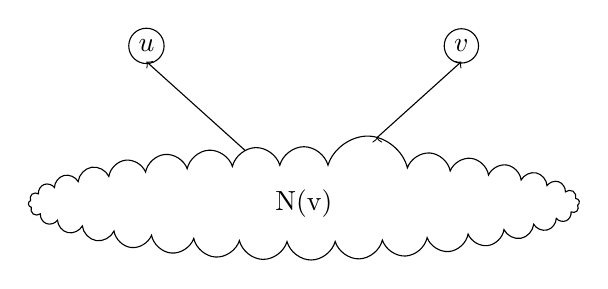
\begin{tikzpicture}
	\node[draw,circle,inner sep=2pt] at (-2, 2) {$u$};
	\node[draw,circle,inner sep=2pt] at (2, 2) {$v$};
	\node[
		name path=cloud,
		cloud, cloud puffs=35.7,
		minimum width=7cm, draw,
		] (cloud) at (0,0) {N(v)};
		\path[name path=path21] (cloud.center) -- (-2, 1.8) coordinate (to21);
		\path[name path=path22] (cloud.center) -- (2, 1.8) coordinate (to22);
		\draw[->,
		name intersections={of=cloud and path21,by=from21},
		name intersections={of=cloud and path22,by=from22},
		] 
		(from21) edge node[at end] {} (to21)
		(from22) edge node[at end] {} (to22)
		;
\end{tikzpicture}
\end{center}

In the above picture, vertices u \& v are non adjacent and shares exact same nieghbourhood graph N(v). Here both u \& v form a partition together.

This property is applicable to complete multipartite graph. Once a vertex in a complete multipartite graph is explored, using this, we can remove all vertices in that partition.

\subsubsection{Two adjacent Vertices shares Same Neighbourhood Graph N(v)}
We can remove all vertices in active graph $G_a$ that has exact neighbourhood graph N(v) as the one searched.

If these vertices are connected then each of the vertex forms a partition.

\begin{center}
	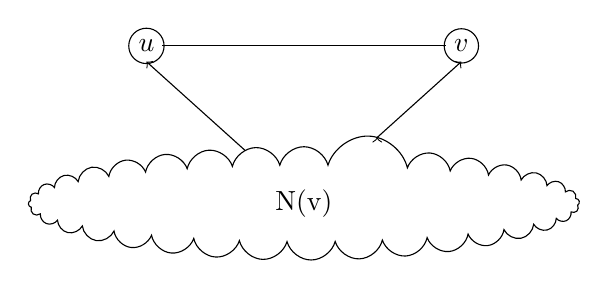
\begin{tikzpicture}
	\node[draw,circle,inner sep=2pt] at (-2, 2) {$u$};
	\node[draw,circle,inner sep=2pt] at (2, 2) {$v$};
	\node[
	name path=cloud,
	cloud, cloud puffs=35.7,
	minimum width=7cm, draw,
	] (cloud) at (0,0) {N(v)};
	\path[name path=path21] (cloud.center) -- (-2, 1.8) coordinate (to21);
	\path[name path=path22] (cloud.center) -- (2, 1.8) coordinate (to22);
	\draw[->,
	name intersections={of=cloud and path21,by=from21},
	name intersections={of=cloud and path22,by=from22},
	] 
	(from21) edge node[at end] {} (to21)
	(from22) edge node[at end] {} (to22)
	;
	\draw (-1.8, 2) -- (1.8,2);
	\end{tikzpicture}
\end{center}

In the above picture, vertices u \& v are adjacent and shares exact same nieghbourhood graph N(v). Here u forms a partition and v forms another partition.

If vertex u's N(v) is searched then vertex v is part of N(v). Similarly if v's N(v) is searched then vertex u is part of N(v).

\subsubsection{Two adjacent Vertices shares Neighbourhood Graph N(v)}

Let u \& v are two adjacent vertices. N(v) of u is \{v, N(v')\}. N(v) of v is \{u, w, N(v')\}. Here in this case, both u \& w forms partition. So, once u explored, we can safely remove both u \& v from active graph $G_a$.

\begin{center}
	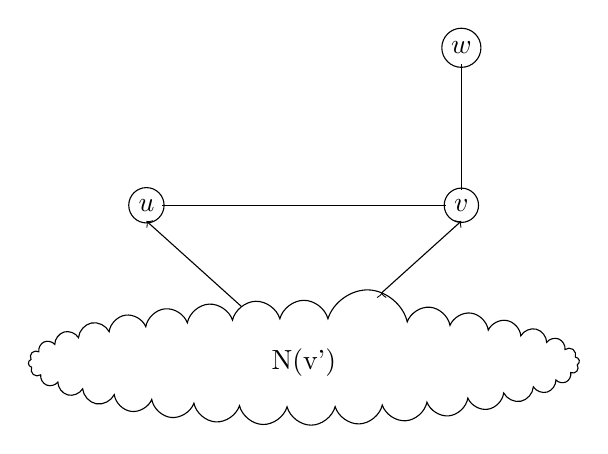
\begin{tikzpicture}
	\node[draw,circle,inner sep=2pt] at (-2, 2) {$u$};
	\node[draw,circle,inner sep=2pt] at (2, 2) {$v$};
	\node[draw,circle,inner sep=2pt] at (2, 4) {$w$};
	\node[
	name path=cloud,
	cloud, cloud puffs=35.7,
	minimum width=7cm, draw,
	] (cloud) at (0,0) {N(v')};
	\path[name path=path21] (cloud.center) -- (-2, 1.8) coordinate (to21);
	\path[name path=path22] (cloud.center) -- (2, 1.8) coordinate (to22);
	\draw[->,
	name intersections={of=cloud and path21,by=from21},
	name intersections={of=cloud and path22,by=from22},
	] 
	(from21) edge node[at end] {} (to21)
	(from22) edge node[at end] {} (to22)
	;
	\draw (-1.8, 2) -- (1.8,2);
	\draw (2, 2.2) -- (2,3.8);
	\end{tikzpicture}
\end{center}


\subsubsection{Two adjacent Vertices shares Neighbourhood Graph N(v)} \label{FenceGraphOptimization}

Let u \& v are two adjacent vertices. N(v) of u is \{v, t, N(v')\}. N(v) of v is \{u, w, N(v')\}. Here in this case, both u \& w forms partition and both v \& t forms another partition. So, once u or v is explored, we can safely remove both u \& v from active graph $G_a$.

\begin{center}
	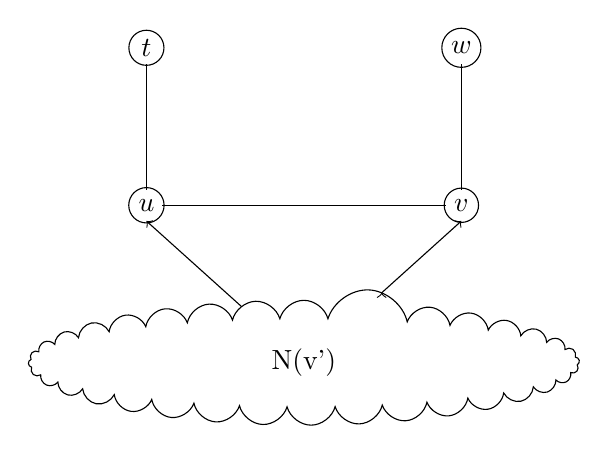
\begin{tikzpicture}
	\node[draw,circle,inner sep=2pt] at (-2, 2) {$u$};
	\node[draw,circle,inner sep=2pt] at (2, 2) {$v$};
	\node[draw,circle,inner sep=2pt] at (2, 4) {$w$};
	\node[draw,circle,inner sep=2pt] at (-2, 4) {$t$};
	\node[
	name path=cloud,
	cloud, cloud puffs=35.7,
	minimum width=7cm, draw,
	] (cloud) at (0,0) {N(v')};
	\path[name path=path21] (cloud.center) -- (-2, 1.8) coordinate (to21);
	\path[name path=path22] (cloud.center) -- (2, 1.8) coordinate (to22);
	\draw[->,
	name intersections={of=cloud and path21,by=from21},
	name intersections={of=cloud and path22,by=from22},
	] 
	(from21) edge node[at end] {} (to21)
	(from22) edge node[at end] {} (to22)
	;
	\draw (-1.8, 2) -- (1.8,2);
	\draw (2, 2.2) -- (2,3.8);
	\draw (-2, 2.2) -- (-2,3.8);
	\end{tikzpicture}
\end{center}

\subsubsection{Neighbourhood Graph N(v) comparison of two adjacent Vertices}
The above two optimization can be generalized as follows. Let u \& v be two adjacent vertices. Now, if N(u) - N(v) forms an independent set and N(v) - N(u) forms another independent set then vertex u forms partition with N(v) - N(u) and vertex v forms patition with N(u) - N(v). So, once either vertex u or vertex v is explored, we can remove both vertices u \& v from active graph $G_a$.

\subsection{Vertex Coloring}
If a graph G can be colored with less than $k$ colors then the graph does not contain a $k$-clique.

As the graph G becomes highly connected, its complement graph G' becomes sparsely connected.


\subsection{Active Graph $G_a$}
As vertices gets explored, the active graph $G_a$ shrinks. The reduction in size of $G_a$ reduces the complexity of exploring remaining neighbourhood graph N(v) of $G_a$. When vertex with minimum degree is explored first, the $G_a$ becomes denser and denser and enables extraction of partition. Also, it enables removal of vertex which shares same neighbourhood graph N(v) of explored vertex as early as possible.

Active graph $G_a$ size is inversely proportional to target clique size that is being searched in terms of complexity. As $G_a$ becomes smaller and smaller against target clique size being mostly constant, remaining search becomes easier and easier.

\subsection{Folding point}
A vertex $v$ can be removed completely from further search once its neighbourhood graph N(v) is completely searched. As we remove explored vertices, active graph $G_a(V-T,E)$ becomes smaller containing only set of vertices that are not yet searched. There comes a point where the remaining active graph $G_a(V-T,E)$ becomes a subset of neighbourhood graph N(v) of one of the already explored vertex. At this point we no longer need to search for maximum clique. The point where the active graph $G_a$ becomes subset of a already explored vertex's neighbourhood graph N(v) is called folding point.

Folding point may occur at any time after at least one vertex is completely explored. For complete multipartite graph, the folding point occurs immediately after exploring all vertices of a single partition.

For clique, the folding point occurs once any vertex's neighbourhood graph is explored.

Hardness of a graph's resistance to this optimization depends on to what extent its each vertex's neighbourhood graph N(v) differs from every other vertex's neighbourhood graph N(v).

\subsection{Vertex \& Edge Constraint}
When searching for clique of size k in graph G(V,E), the graph should contain at least k vertices and each one of these k vertices should have at least (k-1) edges.


\subsection{Picking Vertex with Minimum Degree for Search}
The given undirected graph G(V,E) has single maximum clique size $\omega(G)$ of unknown. The average partition size for the graph G can be calculated by dividing number of vertices it has by its maximum clique size $\omega(G)$. Since not all partitions are going to be same size, picking a vertex with minimum degree results in its neighbourhood graph N(v) being smaller by at least the average partition size. Greater the difference in size between active graph $G_a$ and N(v) of selected vertex with minimum degree, the easier it is to explore. There are couple of reasons for it. One, as the N(v) becomes smaller and smaller, the search space reduces exponentially. Also, while the N(v) becomes smaller, the edge constraint does not relax quickly. This is because, the target clique size k for the next level gets reduced by just one. So the edge constraint becomes tighter against the smaller N(v).

\subsection{Picking Vertex with Maximum Degree for Search}
Does picking a vertex with minimum degree is always better? No. If there exist a vertex with max(deg(V)) whose non-adjacent vertices forms bipartite graph, then picking that vertex reduces time complexity through  \ref{NeighbourhoodGraphOptimization}.

\subsection{Creating Neighbourhood Graph N(v) versus using graph G}
In the recursive algorithm, we have the option to either create and use neighbourhood graph N(v) of the selected vertex, or use input graph G with vertex v's adjacent neighbours as mask. If the algorithm uses input graph G with mask at every level then input graph size $n$ becomes part of time complexity. If neighbourhood graph N(v) is created and used, then average graph size of N(v) at dominating depth (the depth in the recursion that has most number of invokation) becomes part of time complexity.

\subsection{Limit current Neighbourhood Graph N(v) Search using explored neighbourhood graph}\label{AlgorithmOptimizationLimitNodes}

Let current neighbourhood graph be N(v). Pick a neighbourhood graph N(v') from set of explored vertices that intersects N(v) most. During N(v) search, ensure that at least one vertex from N(v) that is not in N(v') is present. Otherwise, we can skip the subgraph if all vertices of it also present in N(v').

\section{Algorithm for checking potential existence of $k$-clique when $N < 2k$} \label{AnyGraph2kFailure}
Let G(V,E) be an undirected graph having N vertices. Let $k$ be the size of clique that is being searched for in G. When $N < 2k$, then we can use the following procedure to check whether k-clique could be present in the graph G or not.

For the graph G to have k-clique, it must have at least k vertices each having at least (k-1) edges.

Let's divide the vertices of G into two groups. To form two groups, first sort the vertices in descending order based on their edge degree. Pick the first k vertices into group A and remaining vertices in to group B.

\begin{align} 
\begin{split}
	\text{Number of vertices in Group A} &= k \\
	\text{Number of vertices in Group B} &= N - k \\
	\text{Let, } \sum_{v \in A} deg (v) \in G(V,E) &= X \\
	\text{Let, } \sum_{v \in B} deg (v) \in G(V,E) &= Y \\
	\sum_{v \in k-clique} deg (v) &= k^2 \\
	\sum_{v \in A} deg (v) \in G(A, E) &= k^2 \\
	\sum_{v \in B} deg (v) \in G(B, E) &= (N-k)^2 \\
	\text{From A to B } &= X - k^2 \\
	\text{From B to A } &= Y - (N-k)^2 \\
\end{split}
\end{align}

For k-clique to be present, the following condition must be met. Otherwise, there is not enough edges in A (after subtracting edges connecting vertices B to A) to form a k-clique. Since we placed top k deg(V) in the first group, grouping them any order will not change the result when it fails.
\begin{align} 
\begin{split}
	\text{Edges connecting vertices A to B} &\ge \text{Edges connecting vertices B to A} \\
	X - k^2 &\ge Y - (N-k)^2 \label{eq:1}
\end{split}
\end{align}

Worst case time complexity for this procedure is $O(n^2)$ due to sorting of vertices based on their deg(V). If the vertices are already in sorted order, then the worst case time complexity is $O(n)$.

\fbox{\parbox{\dimexpr\linewidth-2\fboxsep-2\fboxrule\relax}{
	Satisfying this condition does not mean that k-clique exist. It just means that there is potential for k-clique to exist.
}}

\subsection{Any Graph G(V,E) with k-Clique and $N \ge 2k$ can be converted into G'(V',E') with  k'-Clique such that $N' < 2k'$} \label{AnyGraphTo2k}

\begin{theorem}
	Any Graph G(V,E) with k-Clique and $N \ge 2k$ can be converted into G'(V',E') with  k'-Clique such that $N' < 2k'$
\end{theorem}

\begin{proof}
	Let G(V,E) be a graph with N vertices having k-Clique. Now add a trivial partition (single vertex) to the graph G such that G becomes neighborhood graph N(v) for the newly added vertex v in the trivial partition. (i.e.) An edge is created between every vertex in graph G to single vertex in that trivial partition. The newly created graph G'(V',E') has (k+1)-clique with (N+1) vertices.
	
	If the above procedure is applied (N - 2k + 1) times to graph G(V,E), the resultant graph G'(V',E') with (N + (N - 2k + 1)) vertices and (k + (N - 2k + 1))-clique.
	
\begin{align}
\begin{split}
	N' &< 2k' \\
	N + (N - 2k + 1) &< 2(k + (N - 2k + 1)) \\
	2N - 2k + 1 &< 2k + 2N - 4k + 2 \\
	2N - 2k + 1 &< 2N - 2k + 2 \\
	1 &< 2
\end{split}
\end{align}
\end{proof}

\textbf{This does not invalidate the check. This only incurs the cost of checking when the result would be foregone conclusion. Therefore before applying this check, as many partitions as possible must be extracted to see whether this check can be performed.}

\subsection{Fence Graph}

Fence graph forms complete multipartite graph when $2 \times h + 1 = N$ or $2 \times h = N$ or $2 \times h + 1 = N - 1$. All other cases, we would be applying the above check.

Section \ref{FenceGraphPartition} provides the number of partition a given fence graph will have.

\begin{theorem}
 The equation \eqref{eq:1} will fail for all fence graphs that does not form complete multipartite graph.
\end{theorem}

\begin{proof}
	
\begin{align} 
\begin{split}
\text{Number of vertices in Group A} &= k \\
\text{Number of vertices in Group B} &= N - k \\
\text{Edges of each vertex} &= 2h + 1 \\
\text{X} &= (2h+1)k \\
\text{Y} &= (2h+1)(N - k) \\
\text{Edges connecting vertices from A to B } &= (2h+1)k - k^2 \\
\text{Edges connecting vertices from B to A } &= (2h+1)(N - k) - (N - k)^2 \\
\end{split}
\end{align}

Lets apply above values on equation \eqref{eq:1}.

	
\begin{align} 
\begin{split}
(2h + 1)k - k^2 &\ge (2h+1)(N - k) - (N - k)^2 \\
2hk + k - k^2 &\ge 2hN + N - 2hk - k - N^2 + 2kN - k^2 \\
2hk + k - k^2 &\ge 2hN + N + 2kN - 2hk - k - N^2 - k^2 \\
2hk + k &\ge 2hN + N + 2kN - 2hk - k - N^2 \\
(2h+1)k &\ge 2hN + N + 2kN - (2h + 1)k - N^2 \\
\end{split}
\end{align}

Lets substitue $N = 2 \times k - a$ in above equation.

\begin{align} 
\begin{split}
(2h+1)k &\ge 2h(2k-a) + (2k-a) + 2k(2k-a) - (2h + 1)k - (2k-a)^2 \\
(2h+1)k &\ge 4hk-2ah + 2k-a + 4k^2-2ak - 2hk - k - 4k^2 + 4ak -a^2 \\
(2h+1)k &\ge 2hk + k - 2ah - a + 2ak -a^2 \\
(2h+1)k &\ge (2h+1)k - 2ah - a + 2ak -a^2 \\
0 &\ge 2ak - 2ah - a-a^2 \\
0 &\ge 2a(k-h) - a-a^2 \\
\end{split}
\end{align}

In the above equation $h \& N$ are fixed for the input graph G. $k$ is a variable containing the clique size that we would like to find. As $k$ increases relative to $N$, $a$ also increases to the same amount so that group $B$ reduces accordingly. The minimum difference between $k$ and $h$ is 1 when $a = 1$ ($k = h + 1; 2h+1=N -1$). Therefore right hand side is always a non zero positive value.
\end{proof}

\section{Algorithm for Finding Maximum Clique, Counting and Enumerating Cliques}

The algorithm is to extract partitions from neighbourhood graphs. Each neighbourhood graph is created out of another neighbourhood graph. At minimum, the first element from each partition forms complete multipartite graph. The maximum possible k-partite graph found by this algorithm provides both maximum clique size and an instance of the clique.

To count and enumerate all maximum cliques, extract complete k-partite graph from each found k-partite graph. The sum of product of partition sizes of each complete k-partite graph is the total cliques count while all extracted complete k-partite graph provides all maximum cliques in the graph.


\begin{itemize}
	\setlength{\itemsep}{0pt}
	\setlength{\parskip}{0pt}
	\setlength{\parsep}{0pt}
	\item Algorithm
	\begin{itemize}
		\setlength{\itemsep}{0pt}
		\setlength{\parskip}{0pt}
		\setlength{\parsep}{0pt}
		\item Input
		\begin{itemize}
			\item G(V,E)	: Input graph
			\item k : Default value is 0. To check whether G has k clique then input value is k.
			\item partitions : $\emptyset$
			\item op : Possible operations are Maximum Clique Size; Count Maximum cliques; Enumerate all maximum cliques.
		\end{itemize}
		\item Reference Input for output
		\begin{itemize}
			\item couter : Input value is 0. This tracks the count of maximum cliques
			\item cliques : Input value is $\emptyset$. This tracks all complete k-partite graphs.
		\end{itemize}
		\item Output
		\begin{itemize}
			\item Clique of k size found or not.
			\item If found then the found clique size. $cliqueSize \ge k$
		\end{itemize}
		\item Note: A cost evaluation function can be accommodated to restrict certain branches from being searched for practical use/research. 
	\end{itemize}
\end{itemize}
	

\begin{breakablealgorithm}
	\caption{$Maximum Clique$}
	\begin{algorithmic}[1]
		\Function{MaximumClique}{$G(V,E), k, partitions, op, \& counter, \& cliques$}
		\State $kMax \gets max(k - 1, 0)$
		\State $G_a \gets G$
		\State $SortVertiesInDescendingOrder(V)$
		\While{$(|G_a| > kMax)$}
					\State \Comment{Extract as many partitions as possible}
			\While{$((p \gets ExtractPartition(G_a)) \not\equiv \emptyset)$}
				\State $partitions \gets partitions \cup p$
				\State $G_a \gets G_a - p$
				\State $kMax \gets max(kMax - 1, 0$)
			\EndWhile

			\State \Comment{Process if maximum clique is found}
			\If{($G_a \equiv \emptyset$)}
				\If{($kMax = 0$)}
					\State $k \gets NumberOfPartitionsIn(partitions)$
					\If{($k > currentMaxCliqueSize$)}
						\State $counter \gets 0$
						\State $cliques \gets \emptyset$
					\EndIf
					\State $kPartiteCompleteGraph \gets ExtractCompleteGraph(partitions)$
					\State $counter \gets counter + CliquesCount(kPartiteCompleteGraph)$
					\State $cliques \gets cliques \cup kPartiteCompleteGraph$
				\EndIf
				\State \textbf{break}
			\EndIf

			\State \Comment{Check whether clique is possible when $n < 2kMax$}
			\If{($|G_a| < 2 * kMax$)}
				\State $k_1 \gets |G_a|-kMax$
				\State $E_1 \gets kMax + SumTopVertexEdges(G_a)$
				\State $E_2 \gets k_1 + SumOtherVertexEdges(G_a)$
				\If{(($E_1 - kMax^2) < (E_2 - k_1^2$))}
					\State \Comment{clique does not exist}
					\State \textbf{break}
				\EndIf
				\If{($kMax > FindApproximateVertexColor(G_a)$)}
					\State \Comment{clique does not exist}
					\State \textbf{break}
				\EndIf
			\EndIf

			\State
			\If{($isNearFenceGraph(G_a)$)}
				\State $v \gets PickAVertexWithMaxDegree(G_a)$
			\Else
				\State $v \gets PickAVertexWithMinDegree(G_a)$
			\EndIf
			\State $pp \gets partitions \cup \{v, ...\}$
			\State $G_a' \gets neighborhood(G_a, v, kMax)$

			\If{($|G_a'| \ge kMax$)}
				\State $search \gets (op \textbf{ not in } \{Count, Enumerate\})$
				\State
				\State \Comment{Check current N(v) is subset of already explored vertex}
				\ForAll {$v' \in \{G - G_a\}$}
					\State $G'' \gets neighborhood(G, v')$
					\If{($isSubgraph(G'', G_a')$}
						\State $search \gets false$
					\EndIf
				\EndFor
				\State
				\If {($search$)}
					\State $(found_1, kMax_1) \gets MaximumClique(G_a', kMax, pp, op, counter,  cliques)$
					\If{($found_1$ and (($kMax_1 + 1) > kMax$))}
						\State $kMax \gets kMax_1 + 1$
					\EndIf
				\EndIf
			\EndIf
			\State
			\State $G_a' \gets neighborhood(G_a, v)$
			\State $G_a \gets \{G_a - v\}$
			\State

			\State \Comment{Remove all vertices that has same N(v) as this}
			\ForAll {$v' \in G_a$}
				\State $G'' \gets neighborhood(G_a, v')$
				\If{($isSameOrEquivalent(G_a', G'')$}
					\State $G_a \gets \{G_a - v'\}$
				\EndIf
			\EndFor
		\EndWhile

		\State $kMax \gets |partitions| + kMax$
		\State \textbf{return} $(kMax >= k, kMax)$
		\EndFunction
	\end{algorithmic}
\end{breakablealgorithm}

\section{Time Complexity Analysis}
I do need to learn more to provide precise time complexity for the above algorithm. Because of this, I will try to provide worst case time complexity that would be \textbf{worser than actual} time complexity.

We measure the time complexity in terms of number of vertices in the graph.

\subsection{Time complexity of individual blocks in the algorithm}

\subsubsection{PickAVertexWithMaximumDegree and PickAVertexWithMinimumDegree}
The algorithm sorts the verties in descending order at the beginning. Algorithm retains this order as active graph $G_a$ shrinks.

The worst case time complexity for this step is $O(n^2)$ and once per call.

\subsubsection{Partition Extraction}
The worst case time complexity for this step is $O(n^4)$. Worst case here results in active graph $G_a$ being $\emptyset$. (i.e.) Worst case time complexity is $O(n^3)$ for all complete multipartite graph and $O(n^4)$ for k-partite graph.

Every extracted partition reduces the time complexity of remaining graph. The time complexity is $O(n^2)$ when no partition is extracted.

\subsubsection{When $N < 2k$}
This step is applicable only when active graph $G_a$ becomes smaller enough to satisfy $N < 2k$. The time complexity is $O(n)$. We stop exploring further if we find that there is no potential for k-clique to exist.

\subsubsection{Finding approximate Vertex Color when $N < 2k$}
\textbf{Note: We don't need to find the exact minimum colors needed. We only need to check whether given graph can be colored with at most $k-1$ colors.}

If each vertex is colored with unique color then N colors are needed. If each pair of vertices is colored with unique color then $\frac{N+1}{2}$ colors are needed. To have at least $k$ partitions, the average cardinality of partitions becomes less than 2. Therefore, extracting as many partitions with at least cardinality 3 without compromising the time complexity is enough.

\textbf{Note: The largest partition that can be extracted is less than or equal to difference between N and least vertex degree in the graph G.
}



\subsubsection{Neighbourhood Graph N(v) creation}
Time complexity for creation of neighbourhood graph N(v) is $O(n^2)$.

\subsubsection{Ensuring Neighbourhood Graph N(v) is unexplored one}
Before we explore the neighbourhood graph N(v), we check it is not a subgraph of another already explored vertex. Time complexity for this one is $O(n^2)$.

Note: This needs further study for larger graph since it is possible that the cost may out weigh the benefit.

\subsubsection{Neighbourhood Graph N(v) optimization}
This step is done after a neighbourhood graph N(v) is searched. Using this N(v), we remove list of active vertices that shares the same or equivalent one and reduce the active graph $G_a$. 

Time complexity for this step is $O(n^2)$.

\subsection{Overall Time complexity}
The core of this algorithm is search tree traversal and neighbourhood graph N(v) creation for search.

\subsubsection{Cost of Neighbourhood Graph N(v) creation}
To find this cost, we need to find the call graph depth at which more number of N(v) graphs are explored. The average size of N(v) graphs at this level becomes the cost parameter in worst case time complexity.

\subsubsection{Search Tree Time Complexity}

\subsubsubsection{Complete Multiparite Graph}
All partitions in any complete multipartite graph would be extracted in $O(n^3)$. Therefore the time complexity is $O(n^3)$.

\subsubsubsection{k-partite partition Graph}
This graph is a relaxed version of complete multipartite graph. This graph just needs to satisfy \ref{Partition}. Partition extractor can successfully extract all partitions in $O(n^4)$. Therefore the time complexity is $O(n^4)$.

\subsubsubsection{semi k-partite partition Graph}
This is a graph that contains few partitions that satisfies \ref{Partition}. Remaining part of the subgraph is a random graph where no more partitions can be extracted before the active graph is reduced.

Any partitions that can be extracted would be done in $O(n^3)$. Time complexity for the remaining graph is based on the number of vertices it contains.

Note: The partitions are extracted either through partition extraction at the top of the function or through neighbourhood graph search optimization at the bottom of the function.

\subsubsubsection{Random Graph G with $N < 2k$} \label{TimeComplexityOf2kRandomGraph}
For any random graph G that satiesfies \ref{AnyGraphTo2k} condition, all trivial partitions would be extracted first at $O(n^4)$ and then the remaining graph would be explored as normal random graph G'. Time complexity here depends on the size of remaining random graph.

For any graph that fails the condition \ref{AnyGraph2kFailure}, the time complexity is $O(n)$ since the vertices are already in sorted order.

Satisfying the condition \ref{AnyGraph2kFailure} does not mean that the graph has a k-clique. So we need to search for existence of k-clique.

The graphs that satisfy \ref{AnyGraph2kFailure} has following properties.
\begin{itemize}
	\setlength{\itemsep}{0pt}
	\setlength{\parskip}{0pt}
	\setlength{\parsep}{0pt}
	\item All vertices have at least (k-1) edges. Any vertex that does not have (k-1) edges are already removed from the graph $G_a$.
	\item There are only at most (2k - 1) vertices in the graph $G_a$ and minimum has (k + 1) vertices. If the graph has k vertices and each having (k-1) edges, then it forms a k-clique. 
	\item For there to be k-clique, there must be at least k partitions present.
	\item There is no trivial partition (with one vertex) exist since it is trivial to extract it.
	\item None of the vertices can form independent set with its non adjacent neighbors.
	\item There is no direct multipartite graph. So, all vertices must be connected using different structures or forms.
	\item No partition can be extracted without removing a vertex after exploring.
\end{itemize}

Only two families of graphs can resist extraction of partitions here. One being fence graph families explained here at \ref{FenceGraph} and another one being k-partite graph in complemented form (Clique Sets) mentioned here at \ref{CliqueSet}.

Even though Fence graph(s) resist partition extractions, they fail at evaluation of condition \ref{AnyGraph2kFailure}. Also the fence graph collapses once a vertex is searched for using neighbourhood graph N(v) optimization mentioned here \ref{FenceGraphOptimization} at all levels. This also includes near Fence graphs that has few edges missing to be a proper fence graphs.

Therefore only graphs that resists further partitioning are k-partite complement graphs mentioned in \ref*{CliqueSet} and disconnected graphs. Processing disconnected graphs at this level is polynomial since size of the disconnected graphs are nearly k-clique size.

\textbf{Here after, any further search in neighbourhood graph N(v) of any vertex is going to satisfy \ref{AnyGraphTo2k}.}


Each partition in k-partite graph becomes a clique in complemented graph. It may have at most one k-clique or higher size partition. These graphs have fewer partitions. One or two partition with large size and rest of the partitions being smaller sizes. If the graphs have two or three partitions then it breaks down immediately at next level. If it has more than few smaller partitions then the clique algorithm may take little higher time complexity. But finding vertex colors for these graphs is polynomial since the complement graph is sparse and have smaller maximum cliques. Unless the graph has k-clique, number of colors needed for this graph would be lower than clique size that is being searched. So, if the colors needed is lower than the clique size, then we can stop searching for it.

As we explore minimum vertex, group B in \ref{AnyGraphTo2k} becomes more tighter and collapses the active graph $G_a$.

Due to above reasons and tighter conditions because of vertex with minimum degree selection, and finding colors needed for the graph being polynomial, the time complexity to explore this graph is polynomial. 

\subsubsubsection{Random Graph G(V,E) with $N \ge 2k$} 
All graphs have a fixed maximum clique size $\omega(G)$ of their own. For a graph G with n vertices and $\omega(G)$ clique size, the minimum number of partitions are $\omega(G)$; the maximum number of partitions are n; the upper bound on average partition size is $\frac{n}{\omega(G)}$; the lower bound on average partition size is $\frac{n}{n} = 1$.

The algorithm tries to convert given random active graph $G_a$ into $G'_a$ which could be explored in polynomial time through either as k-partite graph or $n < 2k$ or at least into semi partite graph to reduce size by exploring (searching) as minimum vertices as possible within as smaller amount of time as possible in generic way.

In a way, the algorithm tries to extract partition structures at all levels either before exploring a vertex or after exploring a vertex using its neighbourhood graph N(v).

The depth of search tree is $\omega(G)$. At each depth, the algorithm creates partition with vertex v by creating N(v) for exploring. Any partition extracted at any depth beyond N(v) reduces this depth level by 1.

\paragraph{Larger Partitions}
$\omega(G)$ of graph G directly proportional to number of vertices n and inversely proportional to average partition size. (i.e.) $\omega(G) \approx \frac{n}{averagePartitionSize}$. Therefore, larger the partition size, smaller the number of partitions can be made. Hence graphs with larger partitions have smaller $\omega(G)$ which is directly proportional to search tree depth and smaller time complexity.

\paragraph{Smaller Partitions}
For any graph G, the number of vertices needs to be explored is n - 2k + 1 before the graph $G_a$ could be explored in polynomial time. The approximate number of partitions covered by 2k of graph G with n vertices is $\frac{2 \times k}{averagePartitinSize} = \frac{2 \times k^2}{n}$. Therefore graphs with large number of partitions (having smaller average partition size) has smaller time complexity.

\paragraph{Picking Vertex with Minimum Degree for Search}
At each search tree depth, vertex with minimum degree is picked. This ensures that either the vertex is from a larger partition among the available partitions and/or smaller connected graph among multiple connected graphs. At each depth, the searched clique size gets reduced by 1 while neighbourhood graph N(v) gets reduced by more than average partition size. This reduces the average partition size of remaining partitions. As we go deep in the search tree, the average partition size gets very smaller. This leads to surfacing of of k-partite graph within $G'_a$ and/or it satisfy $n < 2k$ condition.


\paragraph{All Partitions having approximately Equal size}
When a graph has partitions with approximately equal size, and approximately equal number of edges, then they form k-partite graph which has $O(n^3)$ time complexity.

In other words, a graph that has varying size of partitions, varying number of edges and not a k-partite graph is a random graph.

\paragraph{Active Graph $G_a$}
As vertex gets explored and removed from $G_a$, the remaining number of vertices in $G_a$ becomes smaller. Since none of the vertex in $G_a$ can have edges more than the number of vertices in the graph, vertex's edges also gets reduced as its neighbours get removed.

As $G_a$ becomes smaller while vertices gets explored, clique size that is being searched for either remains constant or increases if a larger clique is found. This results in average partition size getting smaller.

\paragraph{Number of Partition versus Partition Size}
The number of partitions in a graph is inversely proportional to partition size. Large number of partitions results in smaller partition size which is relatively easy to explore. Similarly smaller number of partitions results in larger partition size which is also easier to explore. 

Since sum of all partition size equals the number of vertices in the graph, balancing number of partition affects partition size and vice versa. Therefore the worst case time complexity of this algorithm is set at number of partitions ($\sqrt{n}$) being equals to the partition size ($\sqrt{n}$) so that product of number of partitions ($\sqrt{n}$) and partition size ($\sqrt{n}$) equals number of verices (n) in the graph.

\paragraph{Worst Case Time Complexity} The approximate worst case time complexity of search tree is $O(\sqrt{n}$\textsuperscript{$\sqrt{n}$}$)$.
The approximate worst case time complexity for this algorithm is 
$O(\sqrt{n}^2 \times \sqrt{n}$\textsuperscript{$\sqrt{n}$}$) = O(\sqrt{n}$\textsuperscript{$(2 + \sqrt{n})$}$)$.

Note: This algorithm has time complexity of $O(n^3)$ for k-partite graphs. The actual one is lot lower than what is mentioned above.


For n = $2$\textsuperscript{10} = 1024, the above complexity becomes $O(2$\textsuperscript{170}$)$.

\paragraph{Best case Time Complexity}
The best case time complexity of this algorithm is $O(n^2)$ when given graph G is N-clique or singleton partition set (meaning all vertices are independent).

\paragraph{Space consumption}
The algorithm consumes space on the order of $O(n^3)$.

\subsection{Impact of Working Memory Set}
Working set of memory for this algorithm is size of active graph $G_a$. The algorithm runs faster when entire $G_a$ can be stored in CPU cache. The performance impact of when entire $G_a$ couldn't be stored in CPU cache is related to ratio of speed between accessing CPU cache versus system's RAM memory.


\section{Case study}
I would like to provide some metrics of this algorithm against a sample graph. Keller graphs are remarked as some of the hardest graphs in set of samples provided in DIMACS web site. Therefore I wanted to try on one of them. Keller-5 graph has around 776 vertices and hence became sample for trial.

\subsection{Keller-5 graph}
\begin{center}
\begin{tabular}{ll}
	Vertices & 776 \\
	Edges & 225990 \\
	Clique Size & 27 \\
	Graph density for 27-clique & 39\% \\
\end{tabular}
\end{center}

\subsection{Algorithm Statistics}
Note: These statistics were taken using little earlier revision of the algorithm implementation; single thread and no parallelism.

\begin{center}
	\begin{tabular}{lr}
		Wall clock time taken for completion & $2,542,521,999(ms)  \approx 30(days)$ \\
		TryFindClique call count & 703,285,173,499 \\
		Number of times $N < 2k$ \ref{AnyGraph2kFailure} check succeded & 633,190,806,735 \\
		Inner iteration (Edges evaluated) & 1,179,362,341,357  \\
		Identical N(v) eliminations \ref{NeighbourhoodGraphOptimization}  & 495,495,356,392 \\
		Identical N(v) eliminations before N(v) is explored \ref{NeighbourhoodGraphOptimization}  & 1,317,047,970 \\
	\end{tabular}
\end{center}

\subsubsectionbreak

Sum of all calls at each depth of recursion levels is given below.

\begin{center}
	\begin{tabular}{rrr}
		Depth & Calls & Average iterations \\
		1 & 1 & 1\\
		2 & 401 & 401 \\
		3 & 142,948 & 357 \\
		4 & 18,402,772 & 129 \\
		5 & 1,047,840,586 & 57 \\
		6 & 26,427,005,000 & 26 \\
		7 & 249,569,092,300 & 10 \\
		8 & 400,189,686,052 & 2 \\
		9 & 26,026,406,477 &  \\
		10 & 6,596,962 & \\
	\end{tabular}
\end{center}

\subsubsectionbreak
 Even though it took $\approx$ 30 days to complete, in terms of $2^n$, it took only around $\approx 2\textsuperscript{54} $ CPU clock cycles.


\section{Clique Problems - Special Cases}
General clique problem is to find maximum clique size $\omega(G)$ for a randong graph $G$. There will not be any other information provided.

Providing following information speeds up the process of solving clique problem of finding an instance, counting and enumerating instances.

\begin{itemize}
	\setlength{\itemsep}{0pt}
	\setlength{\parskip}{0pt}
	\setlength{\parsep}{0pt}
	\item Does the maximum clique size $\omega(G)$ is available?
	\item Does the number of partition is available?
	\item Does partition details like members are available?
	\item Does relationship between partition members are available?
\end{itemize}

If any of the above information is available then we could make use of these information to speed up the process of finding an maximum clique instance and counting and enumeration of all instances.


\section{Conclusion}

The presented non-combinatorial algorithm provides means to find maximum clique size, maximum cliques, counting all maximum cliques and enumerating all maximum cliques in any arbitrary graph.

The time complexity of algorithm for smaller size of up to 1000 vertices graph is within the reach, and opens up ways to move forward by providing sufficient means to verify, validate, understand and learn things that we could not do before.

Now, instead of qualifying a problem is NP-Hard, we can quantify the hardness of each instances of a problem in graph theory. The needle is moved from classification of combinatorial NP-Hard in to a time complexity that varies from quasi polynomial into sub-exponential into probably exponential based on size of the input.

This also provides enough information for further identifying next level of complexity to find next set of algorithms that could potentially solve problems in near quasi polynomial time.

\section{Acknowledgements}
I would like to thank Wikipedia(https://www.wikipedia.org/) and DIMACS( http://dimacs.rutgers.edu) for the information that are/were made available.

Thanks to all people who put their work on public so that others could learn from it.

%****************************************************************
% Bibliography:
%****************************************************************
\begin{thebibliography}{B-N-R}

\bibitem[{Miller and Muller(1960)}]{MM60}
\textsc{R.~E. Miller and D.~E. Muller}.
\newblock A problem of maximum consistent subsets, 1960.
\newblock IBM Research Report RC-240, J. T. Watson Research Center, New York,
USA.

\bibitem[{Moon and Moser(1965)}]{MoonMoser65}
\textsc{John~W. Moon and Leo Moser}.
\newblock On cliques in graphs.
\newblock \emph{Israel J. Math.}, 3:23--28, 1965.
\newblock \doi{10.1007/BF02760024}.

\bibitem[{Vatter(2011)}]{Vatter}
\textsc{Vincent Vatter}.
\newblock Maximal independent sets and separating covers.
\newblock \emph{American Mathematical Monthly}, 118:418--423, 2011.
\newblock \arxiv{0911.4204}


\end{thebibliography}


\end{document}
